\chapter{Metodolog\'ia}

  Al contrario que en una arquitectura centralizada, en la que la logica de negocio se controla en un sistema
  principal, los servicios en la nube utilizan una arquitectura distribuida, diferentes servicios que se comunican
  entre si para realizar una tarea en conjunto. Los servicios gestionan una coleccion de recursos relacionados
  y exponen su funcionalidad a traves de contratos a otros usuarios y servicios parte del sistema. Esta tipo de
  arquitectura implica una mayor complejidad, al tener que comunicar los diferentes servicios, pero ofrece una
  mayor escalabilidad, tolerancia a fallos y la posibilidad de compartir recursos entre las partes del sistema.

  Seddi ofrece sus servicios a traves de clientes web que exponen la funcionalidad al usuario. El cliente web se
  comunica con un API REST, para gestionar el acceso a recursos compartidos en la plataforma, y una conexion de
  sockets con un sistema de cola de mensajes para pedir y recibir las operaciones graficas mas costosas que se
  realizan en los servidores en la nube.

  \begin{figure}[H]
    \vspace{1cm}
    \centering
      \frame{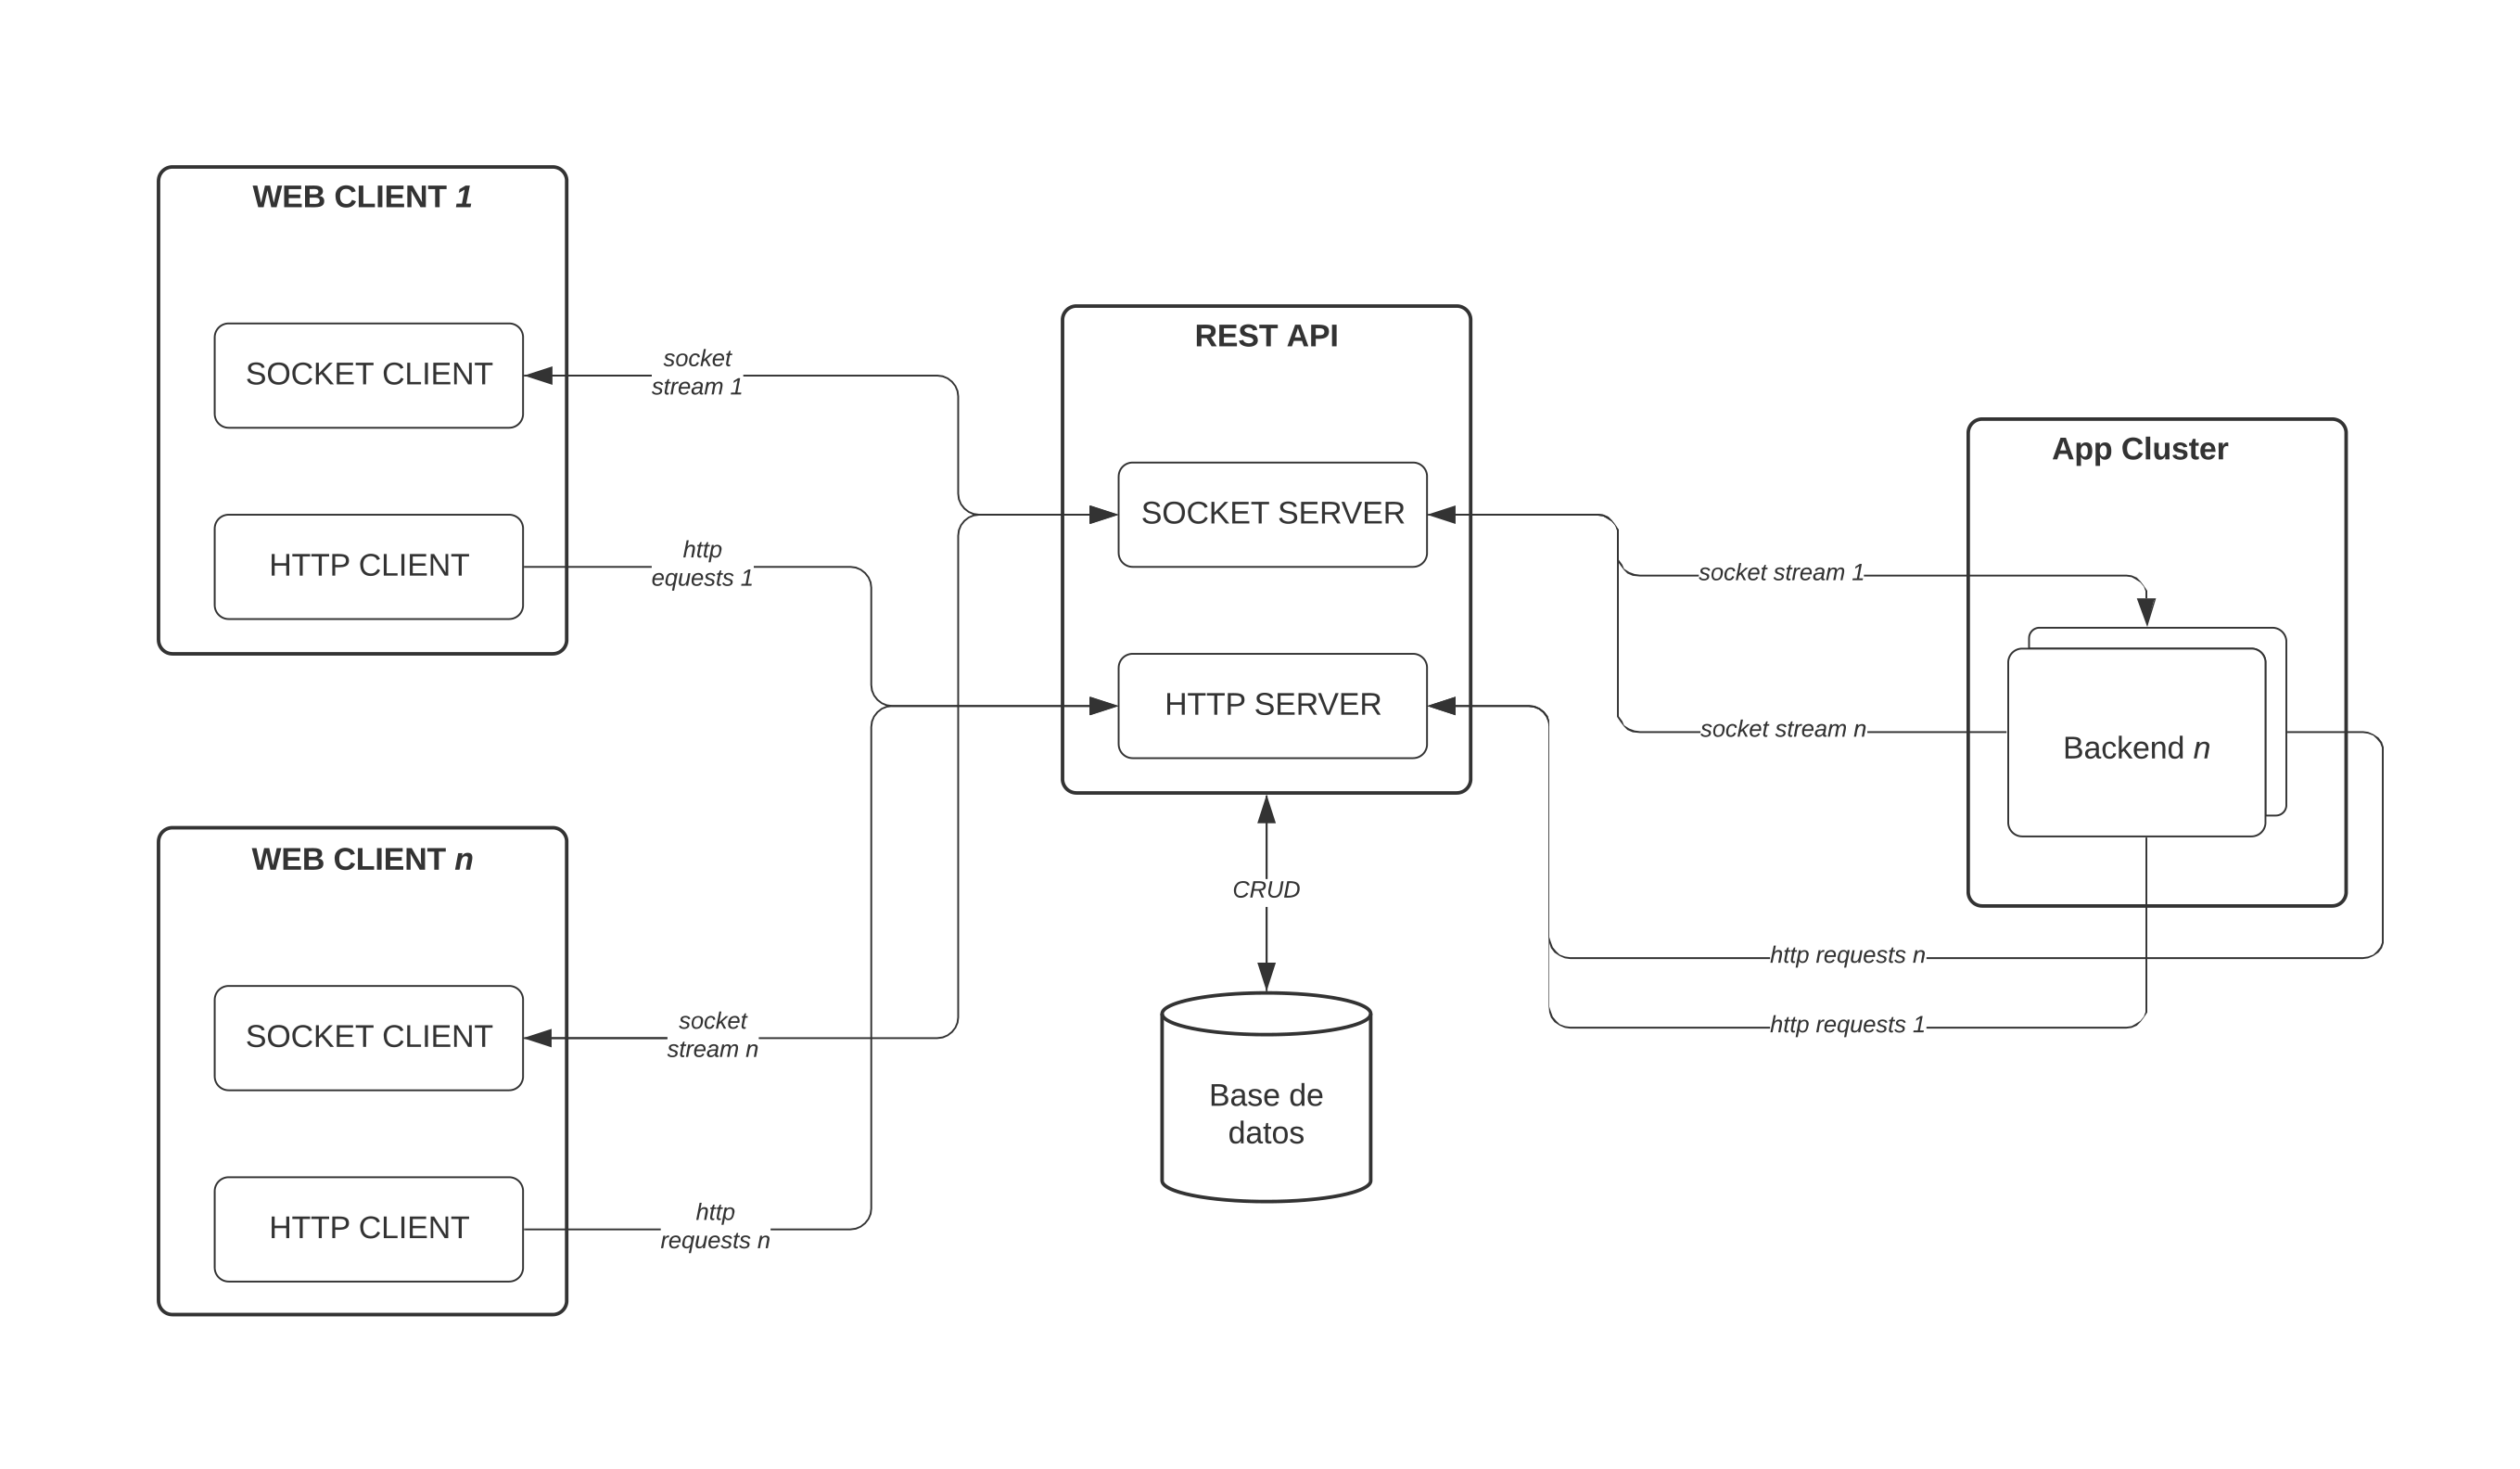
\includegraphics[scale=0.55]{seddi_diagram}}
    \caption{Esquema comunicaciones de servicios en Seddi.}
    \vspace{1.5cm}
  \end{figure}

  En el caso de Author, se trata de una aplicacion web, que utiliza React para la interfaz de usuario, la API de
  Canvas de HTML para el editor 2D y Three.js como motor de render para el editor de 3D. Las interacciones de
  usuario actualizan el estado local del cliente y se comunica con el API REST para persistir los cambios sobre
  los recursos en base de datos. Este flujo permite el disenho y prototipado de la prenda completamente en el
  cliente web, mientras que para las acciones mas costosas, como la simulaci\'on o renderizado offline de tejidos,
  se reserva al usuario un servidor que utiliza un servicio HPC de Seddi encarga de recibir, procesar y enviar la
  peticion a traves del sistema de cola de mensajes.


  \begin{figure}[H]
    \vspace{1cm}
    \centering
      \frame{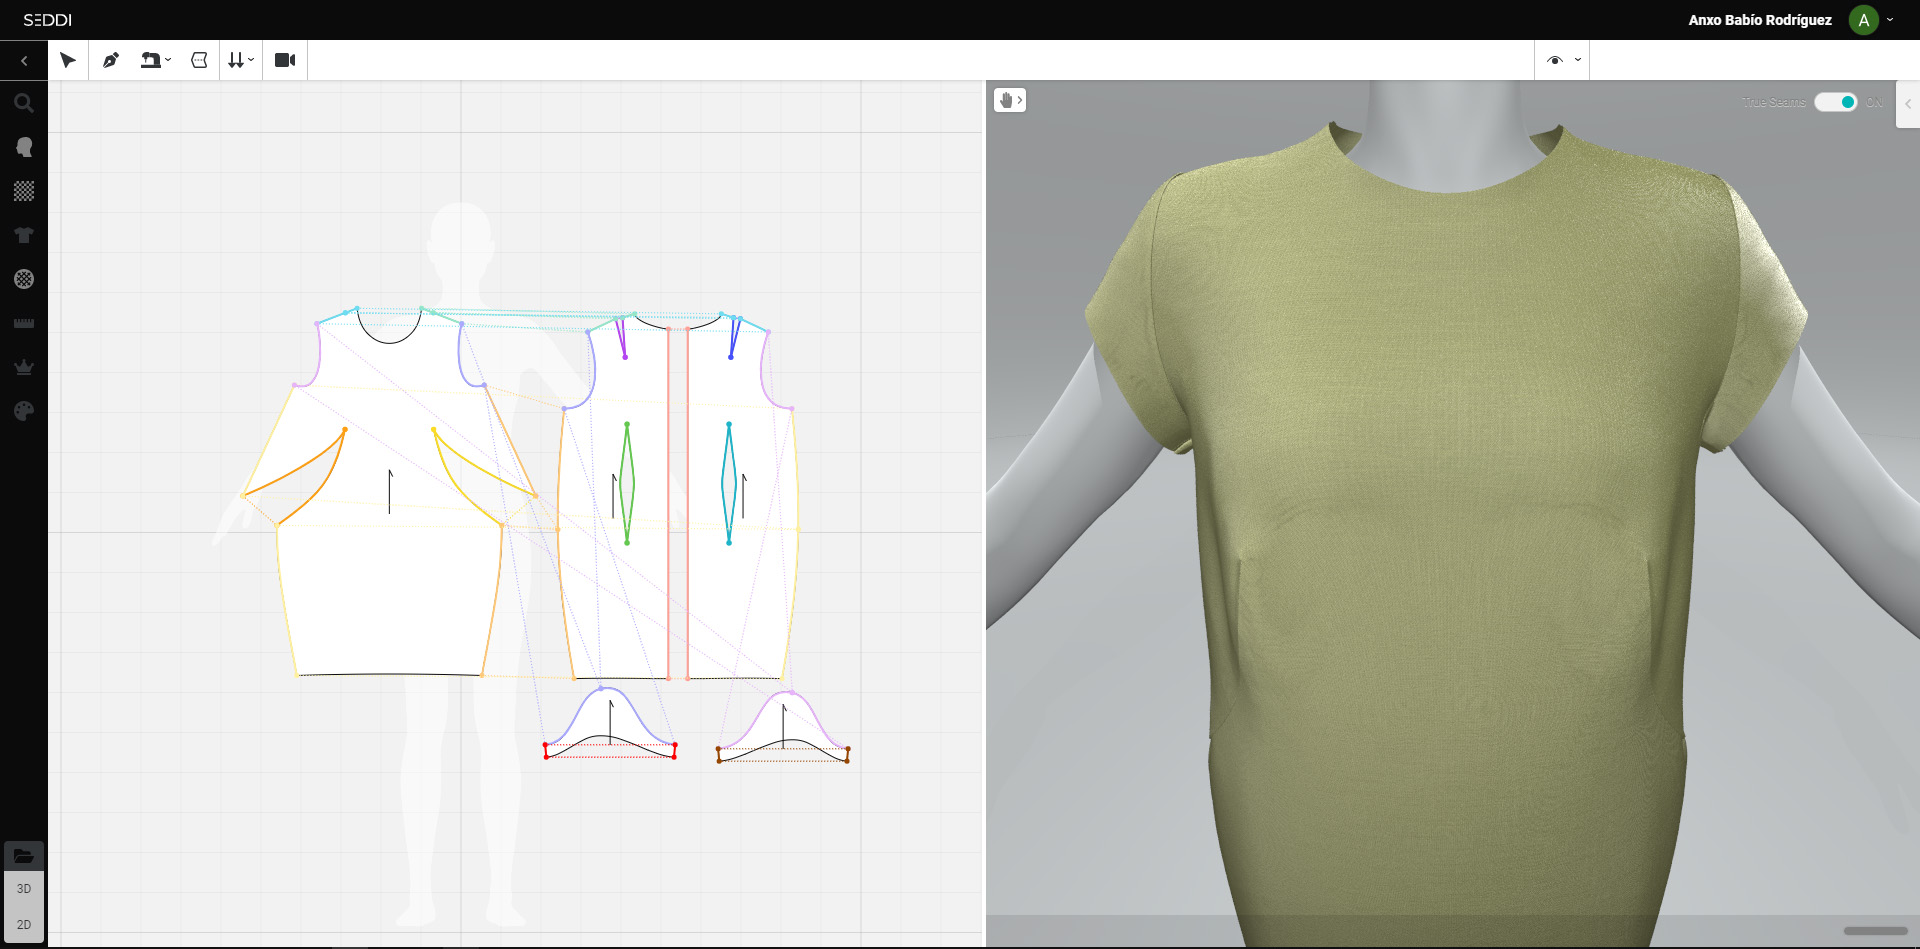
\includegraphics[scale=0.28]{viewports}}
    \caption{Editor de patrones 2D y editor 3D de Author}
    \vspace{0.5cm}
  \end{figure}

  La informacion de un material para que los motores graficos del cliente web y el servicio HPC se almacena en un
  TextureStack, que son resultado de la captura optica de un tejido, o un SurfaceMaterial, la definicion para
  cualquier otro elemento de la escena 3D. Ambos motores graficos utilizan un Entity Component System, por lo que
  la informacion sobre los materiales son una referencia un GarmentPieceComponent, en el caso de un TextureStack,
  o un MeshRenderableComponent, en el caso de un SurfaceMaterial.\\

  Los recursos almacenan diferentes tipos de metadatos, que pueden utilizar diferentes modelos de shading, pero
  comparten la parametrizacion de los materiales. En la figura 4.3 se muestran los esquemas de estos recursos en la
  base de datos.

  \begin{figure}[H]
    \vspace{0.5cm}
    \centering
      \frame{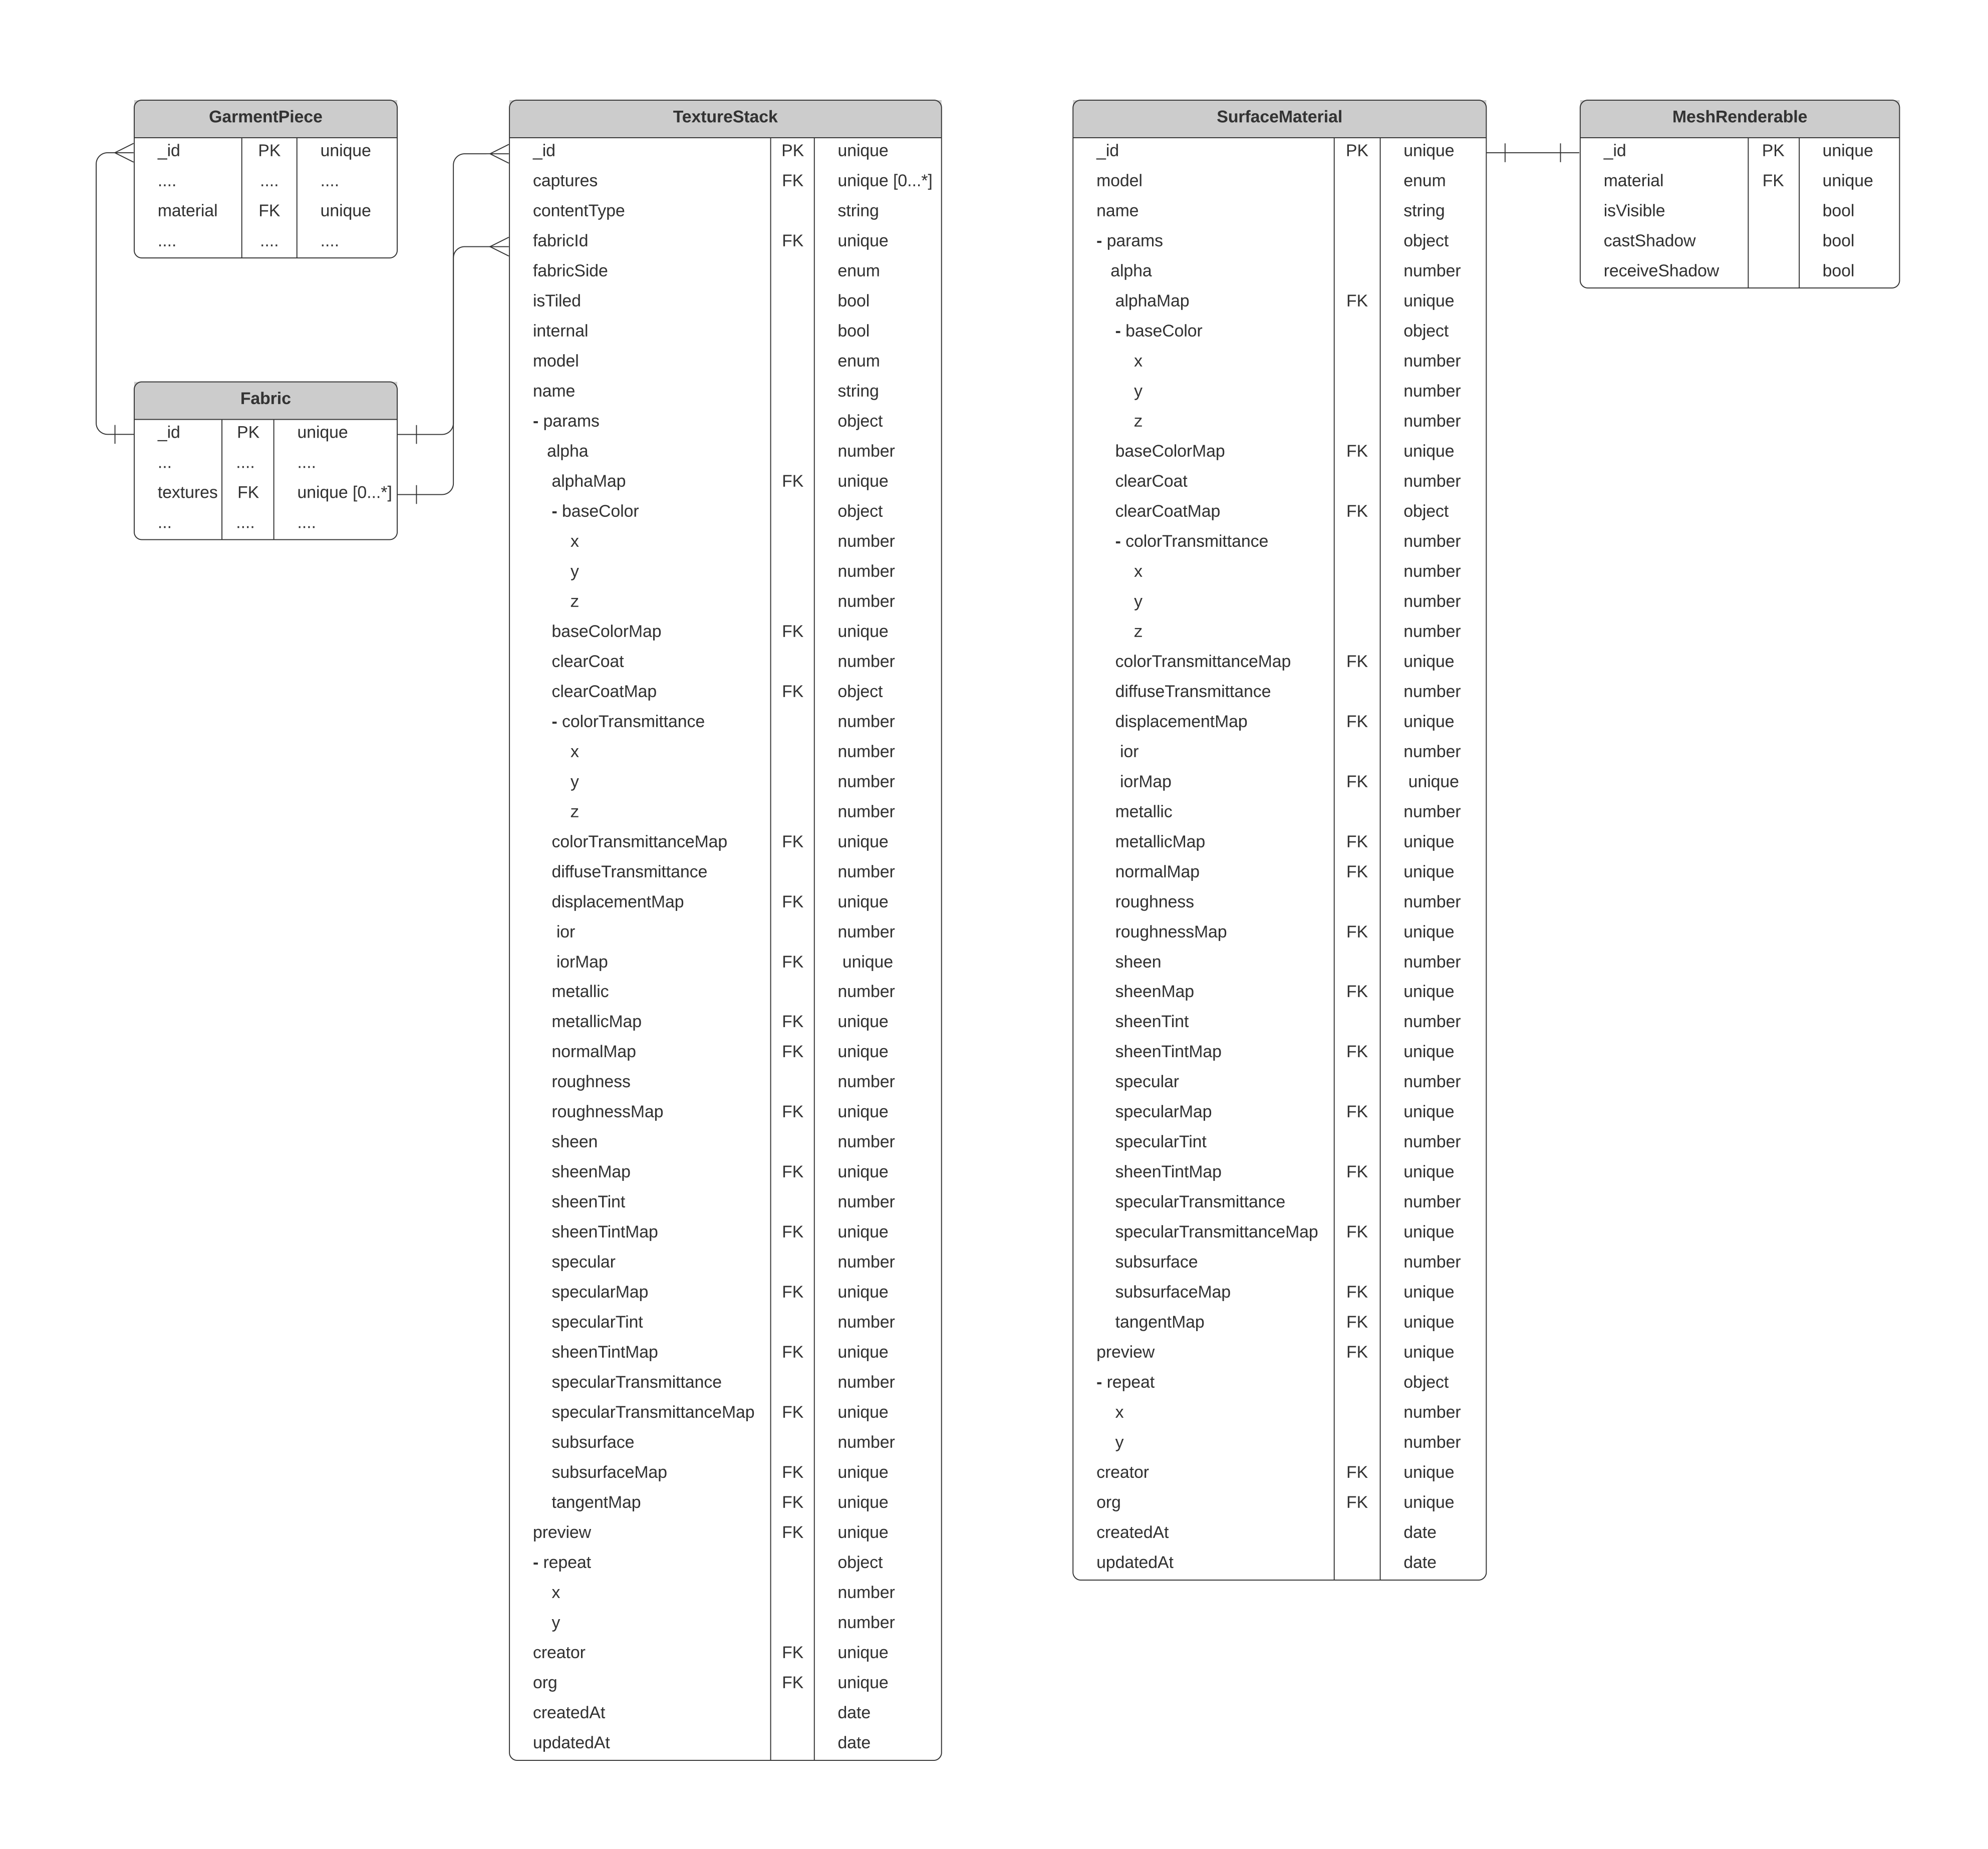
\includegraphics[scale=0.4]{materials_schema}}
    \caption{Modelo de datos de los recursos que utilizan materiales.}
    \vspace{1cm}
  \end{figure}

  El API REST es la interfaz que expone las operaciones disponible sobre este recurso y se documentan con Swagger,
  una herramienta que permite generar documentacion y sirve de guia a los desarrolladores consumidores del API. En
  la figura 4.4 se muestran la documentacion sobre los tipos de peticiones y las rutas del API referidas a recursos
  SurfaceMaterial y TextureStack.

  \begin{figure}[H]
    \vspace{1cm}
    \centering
      \frame{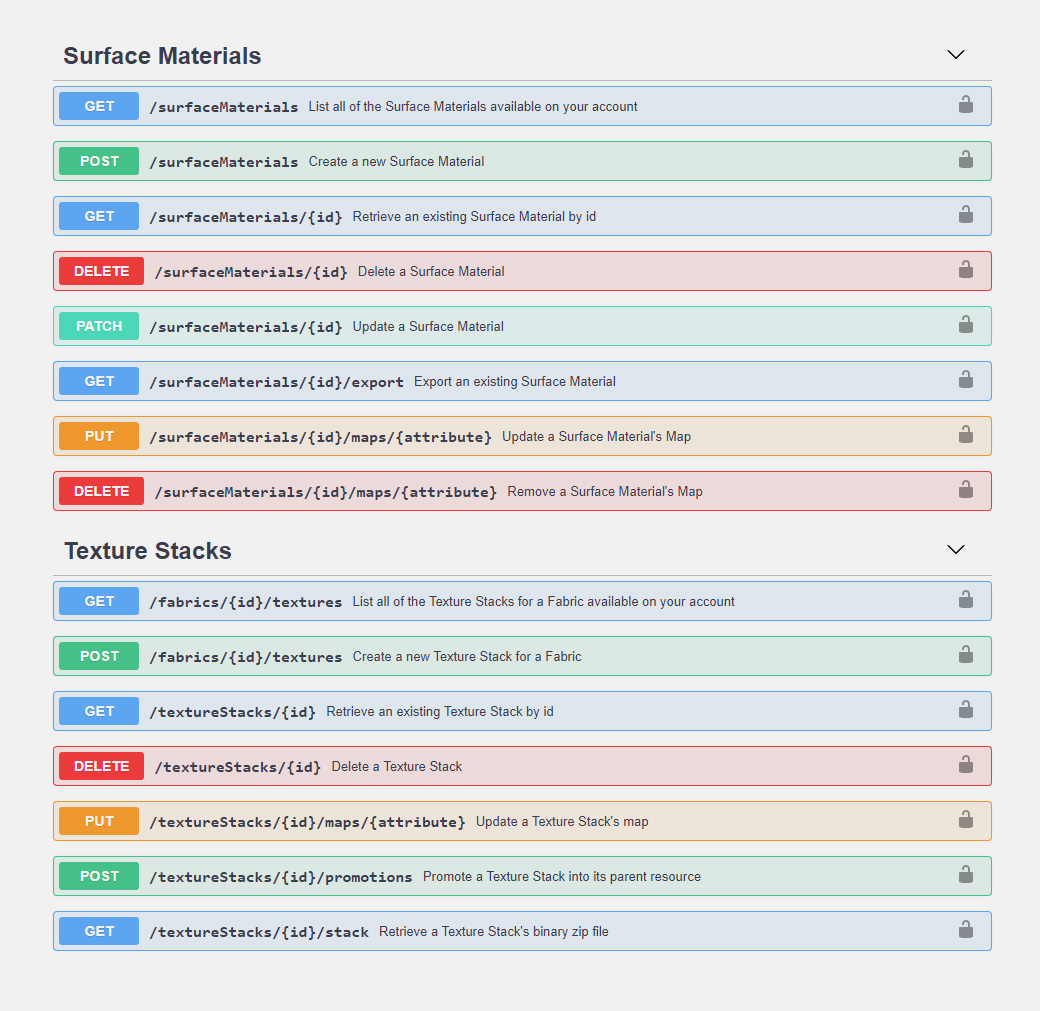
\includegraphics[scale=0.4]{swagger}}
    \caption{Documentaci\'on de los recursos SurafaceMaterial y TextureStack en Swagger.}
    \vspace{1cm}
  \end{figure}